\documentclass[beamer]{standalone}

\usepackage{tikz}

\usetikzlibrary{backgrounds}
\usetikzlibrary{calc}
\usetikzlibrary{positioning}

\definecolor{almost-white}{HTML}{fefefe}


\begin{document}

\begin{standaloneframe}

\begin{tikzpicture}[
    pole/.style={
        draw,
        circle,
        fill=white,
    },
    foo/.style={
        draw,
        rounded corners=.25cm,
        fill=lightgray!25,
        minimum width=1cm,
        inner sep=0,
    },
    dots/.style={
        line width=2pt,
        line cap=round,
        dash pattern=on 0pt off 4\pgflinewidth,
    },
    background rectangle/.style={ draw=almost-white, line width=0pt, },
    show background rectangle,
]



\node [foo, minimum height=6cm] (un) {};
\node [below=of un] (un-label) {\(U_n\)};

\onslide<2->{
    \node [foo, minimum height=4cm, right=2.5cm of un] (un2r) {};
    \node [below=of un2r] (un2r-label) {\(U_{\frac{n}{2}}\)};
    \node [foo, minimum height=4cm, left=2.5cm of un] (un2l) {};
    \node [below=of un2l] (un2l-label) {\(U_{\frac{n}{2}}\)};
    \draw (un-label) -- (un2l-label);
    \draw (un-label) -- (un2r-label);
}

\onslide<3->{
    \node [foo, minimum height=2cm, right=.75cm of un2r] (un2r4r) {};
    \node [below=of un2r4r] (un2r4r-label) {\(U_{\frac{n}{4}}\)};
    \node [foo, minimum height=2cm, left=.75cm of un2r] (un2r4l) {};
    \node [below=of un2r4l] (un2r4l-label) {\(U_{\frac{n}{4}}\)};
    \node [foo, minimum height=2cm, right=.75cm of un2l] (un2l4r) {};
    \node [below=of un2l4r] (un2l4r-label) {\(U_{\frac{n}{4}}\)};
    \node [foo, minimum height=2cm, left=.75cm of un2l] (un2l4l) {};
    \node [below=of un2l4l] (un2l4l-label) {\(U_{\frac{n}{4}}\)};
    \draw (un2l-label) -- (un2l4l-label);
    \draw (un2l-label) -- (un2l4r-label);
    \draw (un2r-label) -- (un2r4l-label);
    \draw (un2r-label) -- (un2r4r-label);
}


% poles
\node [pole, below=.3cm of un.north] (un-0) {};
\node [pole, below=.3cm of un-0] (un-1) {};
\node [pole, below=.3cm of un-1] (un-2) {};
\node [pole, below=.3cm of un-2] (un-3) {};
\node [pole, below=.3cm of un-3] (un-4) {};
\node [pole, above=.3cm of un.south] (un-n) {};
\node [pole, above=.3cm of un-n] (un-n-1) {};
\draw [dots] ($(un-4.south)+(0,-.4cm)$) -- ($(un-n-1.north)+(0,.2cm)$);

\foreach \x in {r,l}{
    \onslide<2->{
        \node [pole, below=.3cm of un2\x.north] (un2\x-0) {};
        \node [pole, below=.3cm of un2\x-0] (un2\x-1) {};
        \node [pole, above=.3cm of un2\x.south] (un2\x-n) {};
        \node [pole, above=.3cm of un2\x-n] (un2\x-n-1) {};
        \draw [dots] ($(un2\x-1.south)+(0,-.4cm)$) -- ($(un2\x-n-1.north)+(0,.2cm)$);
    }

    \foreach \y in {r,l}{
        \onslide<3->{
            \node [pole, below=.3cm of un2\x4\y.north] (un2\x4\y-0) {};
            \node [pole, above=.3cm of un2\x4\y.south] (un2\x4\y-n) {};
            \draw [dots] ($(un2\x4\y-0.south)+(0,-.2cm)$) -- ($(un2\x4\y-n.north)+(0,.1cm)$);
        }
    };
};


\only<1->{
    \node [red, pole, thick] at (un-0.center) {};
    \node [red, pole, thick] at (un-n-1.center) {};
}
\only<1>{
    \draw [-latex, red, thick, dashed, bend left=60] (un-0) to node [right] {?} (un-n-1);
}

\only<2->{
    \node [red, pole, thick] at (un2r-0.center) {};
    \node [red, pole, thick] at (un2r-n-1.center) {};
    \draw [-latex, red, thick, bend left=30] (un-0) to (un2r-0);
    \draw [-latex, red, thick, bend left=30] (un2r-n-1) to (un-n-1);
}
\only<2>{
    \draw [-latex, red, thick, dashed, bend left=60] (un2r-0) to node [right] {?} (un2r-n-1);
}

\only<3->{
    \node [red, pole, thick] at (un2r4l-0.center) {};
    \node [red, pole, thick] at (un2r4l-n.center) {};
    \draw [-latex, red, thick, bend left=30] (un2r-0) to (un2r4l-0);
    \draw [-latex, red, thick, bend left=30] (un2r4l-n) to (un2r-n-1);
    \draw [-latex, red, thick, bend right=30] (un2r4l-0) to (un2r4l-n);
}



\end{tikzpicture}


\end{standaloneframe}

\end{document}
